\chapter{Results}
\label{chap:results}
\section{Object Detection Performance Analysis}
%Present the results of the object detectors, making sure that each setup is clearly defined: architecture, backbone, training hyperparameters, eventual pretraining, etc.
%For each setup we present the performance using AP and AR metrics, their inference times, and the GPU memory usage.

To quantitatively assess the performance of our models and the viability of the proposed training strategies, we evaluated each model configuration using the mean Average Precision (mAP) metric, a standard for object detection tasks. We report mAP at an Intersection over Union (IoU) threshold of 0.50 (mAP@50), which is a common benchmark, as well as the average mAP over IoU thresholds from 0.50 to 0.95 in steps of 0.05 (mAP@50:95) to provide a more comprehensive assessment of localization accuracy. Additionally, we include mAP at a lower IoU of 0.10 (mAP@10) to gauge the models' ability to detect nodules even with less precise bounding boxes.

\subsubsection{NLST Pretraining Results}
First, we present the results of the models trained on the NLST dataset, which served as a pretraining step before fine-tuning on the DLCS dataset.
As mentioned in the previous section, these models are pretrained on the ImageNet dataset, a training from scratch approach would have needed a much larger dataset to achieve comparable results, so we decided to use these weights as a starting point.
The results of the models trained on the NLST dataset are shown in Table \ref{tab:nlst-models}.

\begin{table}[h]
    \centering
    \begin{tabular}{lccc}
        \hline
        \textbf{Model} & \textbf{mAP@10} & \textbf{mAP@50} & \textbf{mAP@[5:95]} \\
        \hline
        \rowcolor{yellow!20}
        RetinaNet ENv2s      & 0.950 $\pm$ 0.015 & 0.756 $\pm$ 0.021 & 0.577 $\pm$ 0.028 \\
        RetinaNet MobileNet  & 0.935 $\pm$ 0.022 & 0.720 $\pm$ 0.029 & 0.560 $\pm$ 0.035 \\
        RetinaNet ResNet50   & 0.889 $\pm$ 0.019 & 0.645 $\pm$ 0.025 & 0.510 $\pm$ 0.031 \\
        FasterRCNN ENv2s     & 0.948 $\pm$ 0.014 & 0.742 $\pm$ 0.020 & 0.577 $\pm$ 0.027 \\
        FasterRCNN MobileNet & 0.908 $\pm$ 0.025 & 0.725 $\pm$ 0.027 & 0.559 $\pm$ 0.033 \\
        FasterRCNN ResNet50  & 0.891 $\pm$ 0.018 & 0.742 $\pm$ 0.019 & 0.546 $\pm$ 0.029 \\
        \hline
    \end{tabular}
    \caption{Object detection performance on the NLST dataset of Faster R-CNN and RetinaNet architectures with different backbones pretrained on COCO.}
    \label{tab:nlst-models}
\end{table}

Surprisingly, the RetinaNet architecture is comparable and, although not statistically significantly better, it presents slightly higher AP metrics compared to Faster R-CNN with the same backbone.
We will see later that this trend is reversed when the models are trained on the DLCS dataset, and from this one might infere that such a difference is due to the difference in difficulty of the datasets, with NLST being easier to detect, we might say that a simpler architecture is sufficient to achieve good results, and that the more complex Faster R-CNN is not able to extract more information from the data.

If we were to compare the results of the other backbones, we can see that the EfficientNetV2S backbone performs the best overall, with the MobileNet backbone beign the second best regardless of its extremely low number of parameters.

This results are also aiming to show that although many architectures are shipped with ResNet50 as a backbone, it is not the best choice for every task, especially when there are available more efficient and effective backbones that already exploit residual connections and other techniques to improve performance.

\subsubsection{DLCS Direct Training Results}
Next, we evaluated the models on the more clinically realistic and challenging DLCS dataset. The models were again initialized with ImageNet1K weights and trained directly on DLCS. This experiment was designed to quantify the difficulty of detecting the smaller, more subtle nodules characteristic of this dataset without the aid of domain-specific pretraining. The results are shown in Table \ref{tab:dlcs-models-not-pretrained}.

\begin{table}[h]
    \centering
    \begin{tabular}{lccc}
        \hline
        \textbf{Model} & \textbf{mAP@10} & \textbf{mAP@50} & \textbf{mAP@[5:95]} \\
        \hline
        RetinaNet ENv2s      & 0.671 $\pm$ 0.058 & 0.427 $\pm$ 0.041 & 0.363 $\pm$ 0.049 \\
        RetinaNet MobileNet  & 0.736 $\pm$ 0.062 & 0.362 $\pm$ 0.044 & 0.352 $\pm$ 0.055 \\
        RetinaNet ResNet50   & 0.678 $\pm$ 0.052 & 0.424 $\pm$ 0.037 & 0.364 $\pm$ 0.045 \\
        \rowcolor{yellow!20} 
        FasterRCNN ENv2s     & 0.745 $\pm$ 0.053 & 0.533 $\pm$ 0.035 & 0.423 $\pm$ 0.043 \\
        FasterRCNN MobileNet & 0.687 $\pm$ 0.059 & 0.337 $\pm$ 0.040 & 0.332 $\pm$ 0.051 \\
        FasterRCNN ResNet50  & 0.679 $\pm$ 0.048 & 0.484 $\pm$ 0.031 & 0.393 $\pm$ 0.039 \\
        \hline
    \end{tabular}
    \caption{Object detection performance on the DLCS dataset of Faster R-CNN and RetinaNet architectures with different backbones pretrained on ImageNet1K.}
    \label{tab:dlcs-models-not-pretrained}
\end{table}

As expected, the performance of the models on the DLCS dataset is significantly lower than on the NLST dataset, reflecting the increased difficulty. As previously announced, now the Faster R-CNN architecture outperforms RetinaNet with EfficientNetV2S and ResNet50 backbones, while the MobileNet still performs better on with the RetinaNet architecture, making it a good candidate for lower-end devices.
The best performing model is the Faster R-CNN with EfficientNetV2S backbone, achieving an overall mAP@50:95 of 0.423, that is still not enough to be clinically useful, although its map@10 of 0.745 shows how it might be used as a screening tool, and that it performs its performance lowers quickly as the IoU threshold increases, which is a common issue with object detection models.

\subsubsection{DLCS Pretrained Results}
Finally, we evaluated the models pretrained on the NLST dataset and then fine-tuned on the DLCS dataset. This approach aims to leverage the larger, more visually distinct nodules in NLST to provide a strong initial feature representation for the more challenging nodules in DLCS, similar to a shallow curriculm learning approach.
The results of the models pretrained on NLST and then fine-tuned on DLCS are shown in Table \ref{tab:dlcs-models-pretrained}.

\begin{table}[h]
    \centering
    \begin{tabular}{lccc}
        \hline
        \textbf{Model} & \textbf{mAP@10} & \textbf{mAP@50} & \textbf{mAP@[5:95]} \\
        \hline
        RetinaNet ENv2s      & 0.665 & 0.404 & 0.343 \\
        RetinaNet MobileNet  & 0.675 & 0.245 & 0.297 \\
        RetinaNet ResNet50   & 0.664 & 0.412 & 0.350 \\
        FasterRCNN ENv2s     & 0.723 & 0.528 & 0.419 \\
        FasterRCNN MobileNet & 0.698 & 0.299 & 0.317 \\
        FasterRCNN ResNet50  & 0.693 & 0.497 & 0.386 \\
        \hline
    \end{tabular}
    \caption{Object detection performance on the DLCS dataset of Faster R-CNN and RetinaNet architectures with different backbones pretrained on NLST (see \ref{tab:nlst-models}).}
    \label{tab:dlcs-models-pretrained}
\end{table}

Unfortunately, the results of this fine-tuning approach are slightly worse than the direct training on DLCS with the ImageNet weights. Although for the best performing model this difference is not statistically significant, it is still a disappointing result.
This might be due to the fact that the NLST dataset is not large enough. Which is a common issue when fine-tuning on a small dataset, as the model might forget useful general features learned from the ImageNet dataset. Despite this problem can be mitigated by using a low learning rate and by freezing some of the layers -- both of which were done in this case -- it is yet a possibility when the dataset is small compared to its complexity. 
On a different note we can see that in this experimental setup the Faster R-CNN performs bettern than RetinaNet on every backbone, with the EfficientNetV2S backbone still being the best performing one.

\subsubsection{Discussion}

The collective results from the NLST pretraining, direct DLCS training, and fine-tuning experiments provide a comprehensive view of the models' capabilities and reveal several key insights into the challenges of lightweight lung nodule detection.

\paragraph{The Superiority of Faster R-CNN on Complex Data.}
A clear and consistent trend emerges when comparing the model architectures across the two datasets. On the simpler NLST dataset, which features larger and more distinct nodules, the lightweight, one-stage RetinaNet performed comparably or even slightly better than the more complex two-stage Faster R-CNN. This suggests that for less challenging detection tasks, the additional architectural complexity of Faster R-CNN provides no significant advantage.

However, this trend completely reverses on the more clinically realistic and difficult DLCS dataset. On this more challenging data, Faster R-CNN consistently and significantly outperforms RetinaNet across all backbone configurations (with the exception of MobileNetV2). This finding strongly suggests that the two-stage approach—with its dedicated Region Proposal Network and second-stage refinement—is better equipped to handle the subtleties and lower signal-to-noise ratio inherent in detecting small, indistinct nodules. It is the more robust and suitable architecture for this specific clinical problem.

\paragraph{The Failure of Domain-Specific Pretraining.}
One of the most surprising outcomes was the ineffectiveness of the pretraining strategy on the NLST dataset. The hypothesis was that pretraining on a large dataset of easier-to-detect nodules would provide a strong, domain-specific feature representation that would boost performance on the more difficult DLCS dataset. The results, however, show the opposite: direct training on DLCS with ImageNet weights yielded slightly better performance than fine-tuning from NLST weights.

This counter-intuitive result is likely attributable to the domain-shift phenomenon and the risk of catastrophic forgetting. The NLST dataset may not be diverse enough or its nodules representative enough of the subtle cases in DLCS. Fine-tuning on a small, complex dataset like DLCS after pretraining on NLST may cause the model to forget the more general and robust low-level features learned from the vast ImageNet dataset. The slight negative impact on performance suggests that, for this specific task, the general-purpose features from ImageNet are more valuable than the specialized features from NLST.

\paragraph{The Optimal Model Configuration.}
Synthesizing these findings, the best performing model configuration for this task is the Faster R-CNN architecture paired with the EfficientNetV2-S backbone, trained directly on the DLCS dataset using ImageNet pre-trained weights. This configuration achieved the highest overall mAP@50:95 of 0.423.

It is important to contextualize this performance. While a mAP of 0.423 represents a strong academic baseline and validates the viability of the lightweight 2.5D approach, it is not yet sufficient for fully autonomous clinical deployment. However, the high mAP@10 score of 0.745 indicates that the model is effective at identifying the general location of potential nodules, suggesting its immediate promise as a ``second reader" or screening tool to draw a radiologist's attention to suspicious areas, which can then be confirmed by expert review. The performance drop at higher IoU thresholds is a well-known characteristic of object detection on small objects and highlights the remaining challenge in achieving perfect localization.

\section{Explainability Performance Analysis}
%Discuss the performance of the explainability methods, comparing them based on the segmentation game, performing some statistical analysis on the results.

To quantitatively evaluate and compare the faithfulness of the adapted explainability methods, the "Inverse Distance Game" (described in Section \ref{subsec:xai_evaluation}) was run on a test set of 819 samples. This section presents the performance of Eigen-CAM, Score-CAM, and Smoothed Score-CAM (SS-CAM), analyzing both their localization accuracy and their computational feasibility.

It is important to note a key aspect of the evaluation protocol: if the object detection model failed to produce any prediction for a given sample, the CAM methods that depend on a baseline output (Score-CAM and SS-CAM) could not be applied. In these cases of detection failure, a score of 0 was assigned to all methods to ensure a fair and consistent comparison across the entire test set.

The comparative results are summarized in Table \ref{tab:xai-inverse-distance} and visualized in the score distribution histogram in Figure \ref{fig:xai-inverse-distance}.

\begin{table}[h]
    \centering
    \begin{tabular}{lrrr}
        \hline
        \textbf{Method} & \textbf{Mean} & \textbf{Std}\\
        \hline
        \rowcolor{yellow!20}
        EigenCAM & 0.90 & 0.12 \\
        ScoreCAM & 0.79 & 0.15 \\
        SSCAM & 0.79 & 0.16 \\
        \hline
    \end{tabular}
    \caption{Inverse Distance results for different XAI methods.}
    \label{tab:xai-inverse-distance}
\end{table}

\begin{figure}[h]
    \centering
    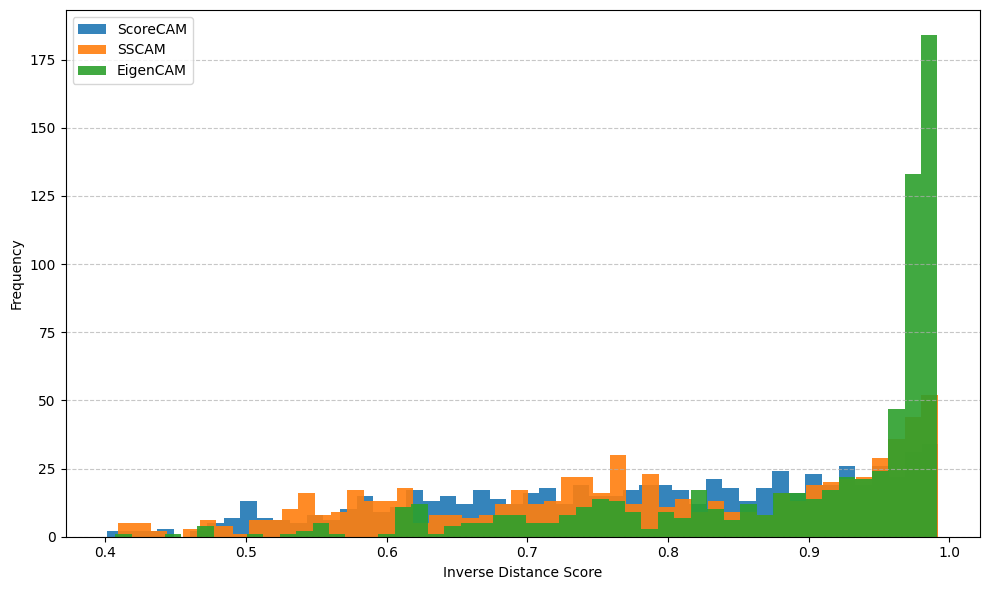
\includegraphics[width=0.8\linewidth]{images/xai-inverse-distance-hist.png}
    \caption{Histogram of the Inverse Distance Game scores for different XAI methods.}
    \label{fig:xai-inverse-distance}
\end{figure}

The quantitative results reveal the clear winner being Eigen-CAM significantly outperforming both Score-CAM and SS-CAM.

To provide a qualitative illustration of these quantitative findings, Figure \ref{fig:xai-qualitative-example} presents a side-by-side comparison of the three methods on a representative sample from the test set. This visual evidence helps to contextualize the numerical scores and provides insight into the behavior of each method.
\begin{figure}[h]
    \centering
    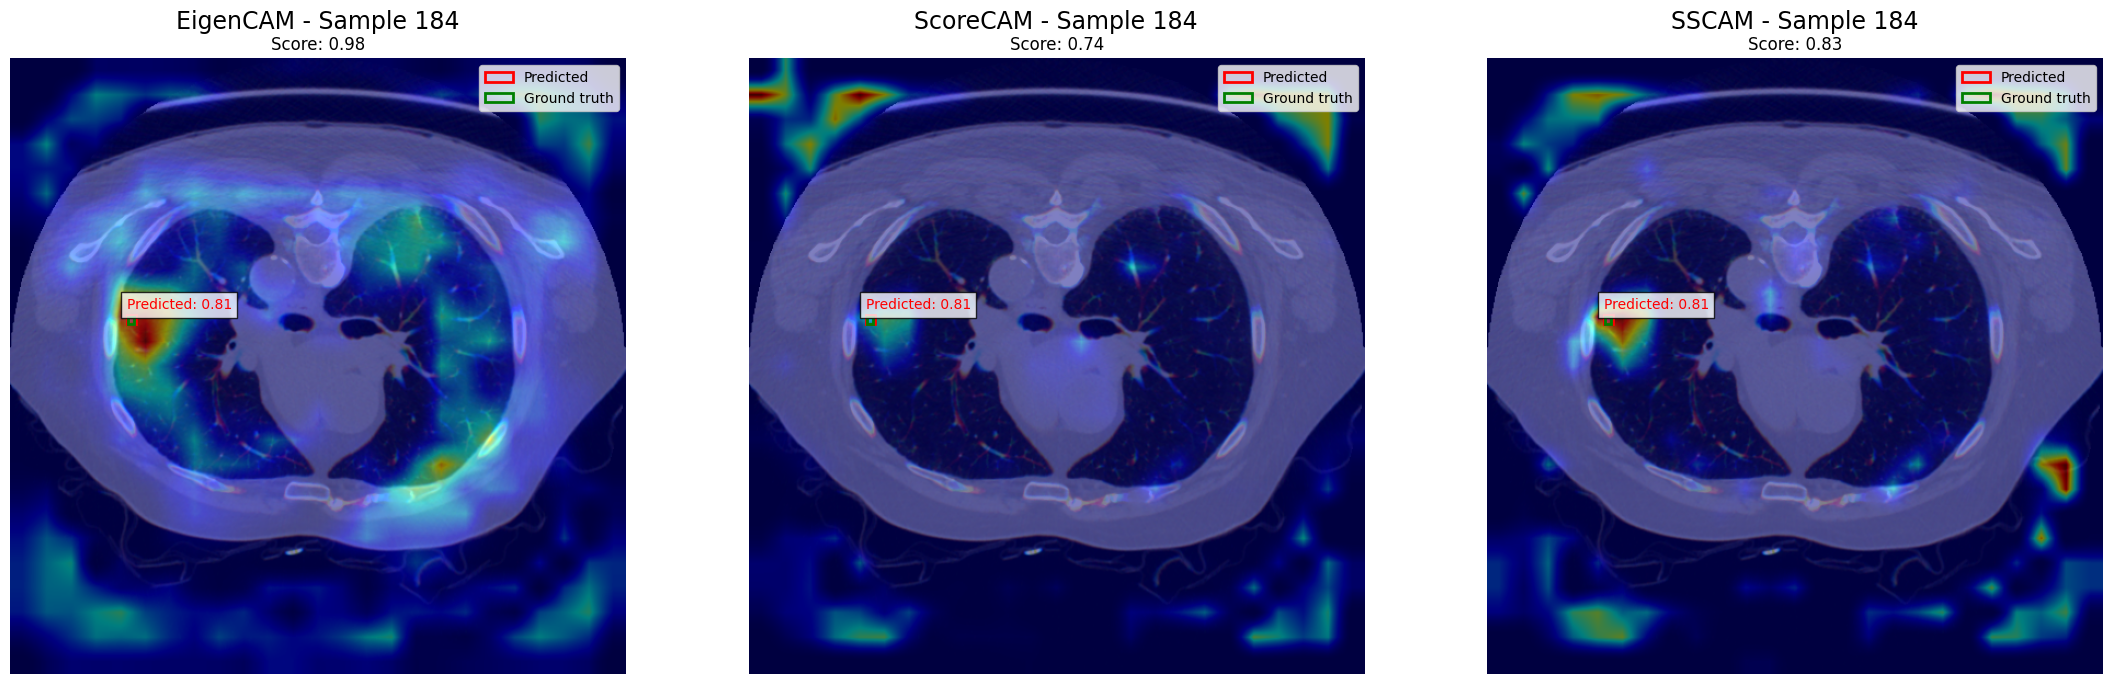
\includegraphics[width=1\linewidth]{images/xai-sample-184.png}
    \caption{Qualitative comparison of CAM methods on a representative test sample (Sample 184). The model's prediction is shown in red, and the ground truth in green. The Inverse Distance Score for each explanation is displayed at the top. \textbf{(Left)} Eigen-CAM, despite producing a heatmap that looks noisier than the others, has its focus right on the nodule (Score: 0.98). \textbf{(Center)} Score-CAM's heatmap has less noise, but its top activations are scattered away from the nodule (Score: 0.74). \textbf{(Right)} SS-CAM shows a minimal smoothing with respect to Score-CAM, but a higher concentration on the point of interest (Score: 0.83)}
    \label{fig:xai-qualitative-example}
\end{figure}

\paragraph{Localization Performance.}
As shown in Table \ref{tab:xai-inverse-distance}, Eigen-CAM achieved a mean Inverse Distance Score of 0.90, substantially higher than the scores of 0.79 for both Score-CAM and SS-CAM. The histogram in Figure \ref{fig:xai-inverse-distance} provides deeper insight into this difference. The distribution for Eigen-CAM is strongly skewed to the right, with a large peak near a score of 1.0. This indicates that for a majority of the test samples, Eigen-CAM's explanation was almost perfectly centered on the ground-truth nodule. In contrast, the distributions for Score-CAM and SS-CAM are much flatter and centered in the 0.7-0.8 range, suggesting their localization is more variable and less precise.

An explanation for this performance gap likely lies in the nature of transfer learning and where each CAM method sources its information. Our detection model is a hybrid: it combines a powerful, pre-trained backbone (EfficientNetV2-S) with randomly initialized, task-specific detection heads that are trained from scratch on our relatively small dataset.
Eigen-CAM operates directly on the activation maps of the FPN, which is the final stage of the backbone. It therefore leverages the rich, robust, and well-generalized features learned from the massive ImageNet dataset. It is, in effect, explaining the output of the most ``mature" part of the network.
Score-CAM and SS-CAM, conversely, must evaluate the model as a whole. They rely on the final output after the data has passed through the less-mature RPN and second-stage heads. These heads, trained only on our limited dataset, may have learned a less stable or ``noisier" function. The performance of these methods is therefore entirely dependent on the custom \texttt{FasterRCNNBoxScoreTarget} metric's ability to interpret these potentially noisy final predictions.
 
From this perspective, Eigen-CAM's success stems from its ability to bypass the potential instability of the task-specific heads and our custom scoring logic. Providing a direct view into the robust feature extractor, which, for a well-trained model, is sufficient to identify the object of interest.

\paragraph{Computational Cost and Practicality.}
The performance difference is further magnified when considering the immense disparity in computational cost:
\begin{itemize}
    \item \textbf{Eigen-CAM:} The entire test set was processed in approximately \textbf{13 minutes}.
    \item \textbf{Score-CAM:} Required approximately \textbf{5 hours} to complete.
    \item \textbf{SS-CAM:} Required approximately \textbf{60 hours}, even with a reduced number of samples (n=10 instead of the conventional n=35).
\end{itemize}

This dramatic difference in runtime has significant practical implications. Eigen-CAM is fast enough to be integrated into an interactive clinical workflow. In contrast, Score-CAM is an offline-only method, and SS-CAM is computationally prohibitive for anything beyond small-scale research experiments (given the current hardware limitations). The fact that the 60-hour SS-CAM procedure offered no performance benefit over the 5-hour Score-CAM suggests that for this task, the smoothing provided by the additional samples was insufficient to overcome the inherent noise of the scoring method. The initial rationale for SS-CAM to be included in this study was to reduce noise originated from such a small dataset, but it seems that this was not the case.

Based on this analysis, Eigen-CAM emerges as the unequivocally superior method for this specific application. It provides more faithful and reliable explanations, as measured by the Inverse Distance Game, while being orders of magnitude more computationally efficient than the adapted Score-CAM variants. For the task of explaining a lightweight, single-class object detector, the simplicity and directness of Eigen-CAM prove to be a significant advantage.


\section{Classification Performance Analysis}
Here we present the results for the classification task, which has been performed using the DLCSD24 extracted patches. For each model we report the F1-Score for both classes. The results are shown in Table \ref{tab:classification-performances}.

\begin{table}[htbp]
    \centering
    \begin{tabular}{lcc}
        \toprule
        % \rowcolor{gray!20} % Highlight the header row
        \textbf{Model} & \textbf{F1-Score (Malignant)} & \textbf{F1-Score (Benign)} \\
        \midrule
        Densenet121      & 0.371 $\pm$ 0.082 & 0.618 $\pm$ 0.051 \\
        MobileNet        & 0.395 $\pm$ 0.075 & 0.629 $\pm$ 0.048 \\
        ResNet18         & 0.608 $\pm$ 0.049 & 0.592 $\pm$ 0.053 \\
        EfficientNetV2s  & 0.418 $\pm$ 0.068 & 0.620 $\pm$ 0.045 \\
        \rowcolor{yellow!20}
        ConvNext-Tiny    & 0.679 $\pm$ 0.038 & 0.690 $\pm$ 0.035 \\
        \bottomrule
    \end{tabular}
    \caption{F1-Scores for Lung Nodule Classification Across Different Models}
    \label{tab:classification-performances}
\end{table}

The results clearly indicate that the ConvNeXt-Tiny architecture achieved markedly superior performance compared to the other models. It obtained the highest F1-Scores for both the malignant class (0.679) and the benign class (0.690). Crucially, these scores are well-balanced, suggesting that the model learned to effectively distinguish between the two classes without significant bias, validating the oversampling strategy for this particular architecture.

The ResNet18 model emerged as the second-best performer, though its scores were substantially lower than those of ConvNeXt-Tiny. It showed a reasonable ability to identify malignant nodules but was less effective on the benign class.

A significant trend was observed among the Densenet121, MobileNetV2, and EfficientNetV2s models. Despite being powerful and efficient architectures, they all exhibited a pronounced performance disparity. While achieving respectable F1-Scores for the benign class (ranging from 0.618 to 0.629), their performance on the malignant class was exceptionally poor (ranging from 0.371 to 0.418). This suggests that, for these specific architectures, even with a balanced training set achieved through oversampling, they failed to learn the complex and possibly more subtle features that characterize malignancy in these cropped patches.

It is important, however, to contextualize these results within the broader goal of clinical applicability. An F1-Score of approximately 0.68, while the best among the tested models, indicates that the task remains challenging with the current limitations and the performance is not yet at a level suitable for direct clinical application. This performance ceiling likely stems from a combination of factors:
\begin{itemize}
    \item \textbf{Inherent Task Difficulty:} The morphological features that differentiate benign and malignant nodules can be extremely subtle, even for trained radiologists, especially on 2.5D patches that lack full volumetric context.
    \item \textbf{Data Limitations:} While oversampling addresses the class count, the absolute number of unique benign nodules is still limited, which can restrict the model's ability to learn a diverse and generalizable set of features.
    \item \textbf{Architectural Constraints:} The use of lightweight, 2D models is a deliberate choice for efficiency, but it may not be sufficient to capture the complex, three-dimensional patterns necessary for highly accurate classification.
\end{itemize}

Therefore, these findings should be interpreted not as a definitive solution, but as an informative baseline. They successfully demonstrate the feasibility of the classification task and, most importantly, identify a promising architectural direction (ConvNeXt-Tiny) that significantly outperforms others. 
